%% BioMed_Central_Tex_Template_v1.06
%%                                      %
%  bmc_article.tex            ver: 1.06 %
%                                       %

%%%%%%%%%%%%%%%%%%%%%%%%%%%%%%%%%%%%%%%%%
%%                                     											      %%
%%  LaTeX template for BioMed Central 						 	      %%
%%     journal article submissions    								      %%
%%                                     											      %%
%%          <8 June 2012>              %%
%%                                     %%
%%                                     %%
%%%%%%%%%%%%%%%%%%%%%%%%%%%%%%%%%%%%%%%%%


%%% additional documentclass options:
%  [doublespacing]
%  [linenumbers]   - put the line numbers on margins

%%% loading packages, author definitions

%\documentclass[twocolumn]{bmcart}% uncomment this for twocolumn layout and comment line below
\documentclass{bmcart}

%%% Load packages
\usepackage{amsthm,amsmath}
\usepackage[nohyperlinks, printonlyused, withpage, smaller]{acronym}
\usepackage{subcaption}
\captionsetup[subfigure]{width=0.9\textwidth}
\usepackage[hyphens]{url}
\usepackage{booktabs}
\usepackage{float}

%\usepackage{hyperref}
%\RequirePackage{hyperref}
\usepackage[utf8]{inputenc} %unicode support
%\usepackage[applemac]{inputenc} %applemac support if unicode package fails
%\usepackage[latin1]{inputenc} %UNIX support if unicode package fails

%%%%%%%%%%%%%%%%%%%%%%%%%%%%%%%%%%%%%%%%%%%%%%%%%
%%                                             %%
%%  If you wish to display your graphics for   %%
%%  your own use using includegraphic or       %%
%%  includegraphics, then comment out the      %%
%%  following two lines of code.               %%
%%  NB: These line *must* be included when     %%
%%  submitting to BMC.                         %%
%%  All figure files must be submitted as      %%
%%  separate graphics through the BMC          %%
%%  submission process, not included in the    %%
%%  submitted article.                         %%
%%                                             %%
%%%%%%%%%%%%%%%%%%%%%%%%%%%%%%%%%%%%%%%%%%%%%%%%%

%\def\includegraphic{}
%\def\includegraphics{}
\usepackage{graphicx}
\graphicspath{ {media/} }

\usepackage{pdflscape}
\usepackage{svg}
\svgpath{ {media/} }

%%% Put your definitions there:
\startlocaldefs
\endlocaldefs

%%% Begin ...
\begin{document}

%%% Start of article front matter
\begin{frontmatter}

\begin{fmbox}
\dochead{Research}

%%%%%%%%%%%%%%%%%%%%%%%%%%%%%%%%%%%%%%%%%%%%%%
%% Enter the title of your article here     %%
%%%%%%%%%%%%%%%%%%%%%%%%%%%%%%%%%%%%%%%%%%%%%%

\title{Impact of COVID-19 Pandemic on Perceived Access and Quality of Care in German People with Parkinson's Disease}

%%%%%%%%%%%%%%%%%%%%%%%%%%%%%%%%%%%%%%%%%%%%%%
%% Enter the authors here                   %%
%%%%%%%%%%%%%%%%%%%%%%%%%%%%%%%%%%%%%%%%%%%%%%

\author[
addressref={aff1},                   % id's of addresses, e.g. {aff1,aff2}
%corref={aff1},                       % id of corresponding address, if any
%noteref={n1},                        % id's of article notes, if any
email={marlena.vanmunster@uni-marburg.de}   % email address
]{\inits{M.v.M.} \fnm{Marlena} \snm{van Munster}}
\author[
addressref={aff1},
%noteref={n1},
email={marcel.printz@uni-marburg.de}
]{\inits{M.P.} \fnm{Marcel} \snm{Printz}}
\author[
addressref={aff1,aff2},
corref={aff1},                       % id of corresponding address, if any
email={david.pedrosa@staff.uni-marburg.de}
]{\inits{D.J.P} \fnm{David J.} \snm{Pedrosa}}


%%%%%%%%%%%%%%%%%%%%%%%%%%%%%%%%%%%%%%%%%%%%%%
%% Enter the authors' addresses here        %%
%%%%%%%%%%%%%%%%%%%%%%%%%%%%%%%%%%%%%%%%%%%%%%

\address[id=aff1]{%                          % unique id
\orgdiv{Department of Neurology},             % department, if any
\orgname{Philipps University},          % university, etc
\city{Marburg},                              % city
\cny{Germany}                                    % country
}

\address[id=aff2]{%                          % unique id
\orgdiv{Centre of Mind, Brain and Behaviour},             % department, if any
\orgname{Philipps University},          % university, etc
\city{Marburg},                              % city
\cny{Germany}                                    % country
}

%%%%%%%%%%%%%%%%%%%%%%%%%%%%%%%%%%%%%%%%%%%%%%
%%                                          %%
%% Enter short notes here                   %%
%%                                          %%
%% Short notes will be after addresses      %%
%% on first page.                           %%
%%                                          %%
%%%%%%%%%%%%%%%%%%%%%%%%%%%%%%%%%%%%%%%%%%%%%%

\end{fmbox}% comment this for two column layout

%%%%%%%%%%%%%%%%%%%%%%%%%%%%%%%%%%%%%%%%%%%%%%%
%%                                           %%
%% The Abstract begins here                  %%
%%                                           %%
%% Please refer to the Instructions for      %%
%% authors on https://www.biomedcentral.com/ %%
%% and include the section headings          %%
%% accordingly for your article type.        %%
%%                                           %%
%%%%%%%%%%%%%%%%%%%%%%%%%%%%%%%%%%%%%%%%%%%%%%%

\begin{abstractbox}

\begin{abstract} % abstract
\parttitle{First part title} %if any
Text for this section.

\parttitle{Second part title} %if any
Text for this section.
\end{abstract}

%%%%%%%%%%%%%%%%%%%%%%%%%%%%%%%%%%%%%%%%%%%%%%
%% The keywords begin here                  									      %%
%%%%%%%%%%%%%%%%%%%%%%%%%%%%%%%%%%%%%%%%%%%%%%

\begin{keyword}%three to ten keywords
\kwd{Parkinson's disease}
\kwd{\textsc{Covid}-19 pandemic}
\kwd{health care}
\kwd{impact}
\kwd{influence}
\kwd{Germany}
\kwd{iCARE-PD}
\end{keyword}

\end{abstractbox}
%\end{fmbox}% uncomment this for two column layout

\end{frontmatter}

%%%%%%%%%%%%%%%%
%% Background 		      %%
%%%%%%%%%%%%%%%%

\section*{Background}
The \textsc{Covid}-19 pandemic has presented societies with unprecedented challenges. The uncontrolled spread of a virus causing potential fatal side effects despite intensive care and the consecutive necessity to reduce everyday life has afflicted societies economically and culturally. Yet, the impact on healthcare systems was particularly drastic. With rising incidences, public life around the world came to a standstill and access to public services, including healthcare, were limited to the most basic needs. This standstill has affected individuals in societies differently: vulnerable groups, such as people with chronic illnesses, were particularly affected by the restrictions \cite{sepulveda2020impact, kasar2021lif, yogev2021covid}. This is not overly surprising insofar as that chronic illnesses affect individual psychosocial functioning negatively \cite{demirtepe2022psychosocial}, thus people with chronic illnesses are often dependent on social, financial or physical support. Additionally, people with chronical illnesses often require continous non-emergency medical services and seemed therefore at high risk of undersupply during the pandemic. 

The group of the chronically ill also includes people with \ac{pd}. Person´s living with \ac{pd} show a progressive condition characterized by motor but also non-motor symptoms. A plethora of different clinical signs may emerge during the course of \ac{pd}, which is why  continuous therapy adjustments and needs assessments by healthcare professionals are required. Several studies have unveiled the impact of the \textsc{Covid}-19 pandemic on person´s with \ac{pd} \cite{yogev2021covid, zipprich2020knowledge, frundt2022impact, richter2021analysis, brooks2021social}. What remains unclear, however, is whether all patients were equally affected by the \textsc{Covid}-19 crisis.

Studies from other areas of public health research indicate very indicidual affection of public health crisis \cite{huijts2017prevalence, lowcock2012social}. With regard to \ac{pd}-patients individual symptoms may play an important role, but more generally, this inequality can also be explained by so-called \ac{sdh}. \ac{sdh} are non-medical factors that influence, among other things, peoples access to healthcare, these factors can be present at both individual and societal level \cite{world2010conceptual}. The link between \ac{sdh} and individuals access to healthcare is observable with regard to the \textsc{Covid}-19 pandemic, which means that some population groups experienced greater impacts than others based on their \ac{sdh} \cite{whocovidbrief}. People with \ac{pd} in particular are dependent on a good social support network, which raises the question of whether patients with poorer \ac{sdh} were affected more severly by the \textsc{Covid}-19 crisis.

What may be considered as relevant \ac{sdh} is by no means universal. Rather, a context-specific consideration is required \cite{world2010conceptual}. For \ac{pd}, Zaman et al. proposed a model summarising structural and individual factors potentially influencing patients access to healthcare \cite{zaman2021barriers}. Structural \ac{sdh} may thereby be encompass barriers, that \ac{pd}-patients meet on a system-level when accessing healthcare, such as a lack of care coordination, limited communication between healthcare providers, disparities in health services or the unavailability of specialised services \cite{zaman2021barriers}. Personal barriers, influencing \ac{pd}-patients abilities  to seek help, engage with care providers, reach important care services or pay for them \cite{zaman2021barriers} may, in turn, pose individual \ac{sdh}.

To our knowledge, it has not yet been investigated how \ac{sdh} may relate to the \textsc{Covid}-19 pandemic on PD-patients access to healthcare. Therefore, we examined the impact of a multitude of factors on people suffering from \ac{pd} with special emphasis on their access to healthcare during the pandemic in Germany. 

\newpage
%%%%%%%%%%%%%%%%
%% Methods %%
%%%%%%%%%%%%%%%%

\section*{Methods}
Analyses rely on an anonymous survey carried out as part of the \ac{icarepd}-project (\url{https://icare-pd.ca/}). Witin the scope of the project, a 49-items questionnaire was developed which aimed at characterising the access of \ac{pd}-patients to healthcare services prior and during the pandemic. The initial questions in English were translated to German and were structured in four sections: A) questions describing patients' health status (in terms of \ac{pd} but also of concomitant diseases), B) questions regarding experiences with healthcare services within twelve months before the pandemic, C) questions addressing experiences with healthcare services during the \textsc{Covid}-19 pandemic with special emphasis on telemedicine services, and, D) questions devoted to ascertain demographic backgrounds of participants. There were single, multiple choice questions or open-ended quesions, some of which depended upon the specific answers on previous ones. A full version of the questionnaire is included in the supplementary material. 

The questionnaire was distributed nationwide using the members’ e-mail newsletter of the German Parkinson Association (\ac{dpv}) between November 2020 to January 2021. The e-mail included a short inivtation as well as a link to an online survey, which patients could access using a personal computer, a tablet or a smart phone. In Germany, SoSci Survey \cite{leiner2016} served as database for hosting the survey. Throughout the data inout, the database was supervised and manually checked for plausibility. 

In addition to Germany, the \ac{icarepd} questionnaire was also shared with patient associations in Canada, Spain, Portugal and the Czech Republic with the respective translations. In this study, we limit ourselves to data collected from German patients. 


\iffalse
%trifft davon etwas zu?
% DP: was meinst Du? Oder habe ich das geschrieben?
Questionnaires with inconsistent answers (n = XY) or >XY percent of missing data (n = XY), were excluded from analysis.
\fi

\subsection*{Statistical analyses}
%könnte man die 2 Fragen in eine Art Tabelle oder Box packen?
All analyses were conducted in R (R Core Team (2021), \cite{rcore}). After estimation of descriptive statistics, satisfaction with overall \ac{pd}-related care was compared before and during the pandemic using a non-parametric \textit{sign-test} (rstatix package, \url{https://github.com/kassambara/rstatix/}). The two questions that were used were: ``In the 12 months prior to the COVID-19 pandemic, overall, how satisfied are you with the way healthcare services related to Parkinson’s disease were provided?'' (B17) vs. ``Since the beginning of the COVID-19 pandemic, overall, how satisfied are you with the way healthcare services related to Parkinson’s disease are provided?'' (C6). 

Furthermore, using a \ac{glm} we estimated the odds for worse satisfaction with \ac{pd}-related care. After establishing the full model with a total of 32 predictors, we conducted a stepwise logistic regression in order to reduce the complexity leaving the most meaningful predictors for the question: ``Since the beginning of the \textsc{Covid}19 pandemic, how often did you feel you needed healthcare for Parkinson’s disease but did not receive it?'' (C4). For that purpose, first missing data was imputed taking advantage of a multivariate imputation scheme using the \textsc{Mice}-package \cite{vanBuuren2011}. We thereby assumed data missing at random and used the \ac{pmm}. After missing data imputation, stepwise reduction using a \ac{glm} with Stepwise Feature Selection (\textit{glmStepAIC}) in both directions from the \textit{caret}-package aimed at minimising the \ac{aic}. For that, we first split all data into 80\% of training and 20 \% of test data and performed the stepwise regression after centering and rescaling values and applying a 10-fold cross-validation. The predictions of the two models were compared with the test data using Accuracy, \ac{auc} and LogLoss as metrics. All data for the analyses and all analyses can be followed under \url{https://github.com/dpedrosac/covidPD/}

\subsection*{Additional data}
Within the last section of the survey, participants were asked to disclose the first three of five numbers of their German postal code, which allowed for regional data containment. We concatenated resulting data with publicly available population densities\footnote{\url{https://www.bbsr.bund.de/BBSR/DE/forschung/raumbeobachtung/Raumabgrenzungen/deutschland/regionen/Raumordnungsregionen/raumordnungsregionen-2017.xlsx?\_\_blob=publicationFile\&v=3}} and those for family doctors and neurologists\footnote{\url{https://gesundheitsdaten.kbv.de/cms/html/16402.php}}. Merging the available data with the maps for postal codes\footnote{\url{https://www.suche-postleitzahl.org/downloads}} resulted in maps (cf. Figure \ref{fig1:total}). Densities were stratified into five equal quantiles to allow for analyses. Moreover, the provided information of concomitant diseases (besides \ac{pd}) was collated to a score -- the Elixhäuser Comorbitiy Score with its modification introduced by van Walraven et al. \cite{van2009modification}; here, higher values indicate more severe disease burden. Finally, all questions were assigned to barriers to accessing health services regarding \ac{pd} as described by \cite{zaman2021barriers} (cf. Table \ref{tab3:matchingzaman} supplementary data).

\newpage
%%%%%%%%%%%%%%%%
%% Results %%
%%%%%%%%%%%%%%%%

\section*{Results}
In total, 551 questionnaires were filled out with 252 different postal codes from all 17 German regions (Bundesländer, cf. Figure~\ref{fig1:total}A). Of all participants, 388 (70.4$\%$) returned a complete questionnaire (for demographics from parts A and D of the questionnaire cf. Table~\ref{tab1:demographics}). 

Satisfaction for PD-related care significantly decreased during the pandemic. Hence, the \textit{sign-test} for the question: ``Overall, how satisfied are you with the way healthcare services related to \acl{pd} are provided?'' indicated lower values during the pandemic (Mdn = 1) compared to before (Mdn = 3, \textit{p} = 10\textsuperscript{-73}). More than 90\% of all participants stating to be rather unsatisfied or very unsatisfied with their \ac{pd}-related care during the pandemic (cf. Figure \ref{fig2:satisfaction}). 

To ascertain underlying reasons for dramatic declines of satisfaction, logistic regressions on question C4 (`Since the beginning of the \textsc{Covid}-19 pandemic, how often did you feel you needed healthcare for \acl{pd} but did not receive it?'') was performed unveiling different factors which contributed to this perception of unmet neets during the pandemic (cf. Figure \ref{fig3:resultsOR1}). Thus odds to affirm this question were highly significant (\textit{p} $<$ .001) for those patients inferring lower levels of competence for their neurologist, with a lower ability to access \ac{pd}-care before the pandemic, for patients with higher degrees of stigmatisation in healthcare and for those who did not receive healthcare services before the pandemic. A significant contribution -- albeit lower with significance values \textit{p} $<$ .05 --  were encountered for \ac{pd}-patients with increasing levels of comorbidity, with perceived lower expertise of the \ac{gp}, with higher quality of life scores retrospectively, for people with higher financial burden due to \ac{pd} or who rescheduled healthcare due to financial burden before the pandemic. Finally, lack of availability of remote healthcare during the pandemic and geographical or in general more numerous barriers before start of the pandemic were also indicative of higher odds to perceive unmet needs. For an illustration on significant predictors cf. Figure \ref{fig3:resultsOR1} and for the entire list of results cf. Table  \ref{tab4:resultsall} in the supplementary material. 

%MvM:  Einige der Items verstehe ich ehrlicherweise nicht ``rescheduled healthcare due to financial burden before the pandemic ??! DP:Ich auch nicht. Aber vielleicht habe ich das falsch übersetzt. Marlena, kannst Du vielleicht mal bei den Ergebnissen schauen, welche Werte das waren und wie man die sonst übersetzen würde?

Starting with the entirety of 32 questions that might be predictors of affirming question ``C4'' (see above), using a two-way stepwise regression model these could be reduced to 7 which were: Educational level, Perceived GP's experience, Confidence in assessing necessary services remotely, Ease obtaining healthcare prior to the pandemic, Ability to assess care prior to the pandemic, the density of neurologists and the ability to overcome bassiers (cf. Table \ref{tab2:reduced_model}). Markers for model comparison were indicative of similar performances in the ``full model'' with 32 predictors compared to the reduced one (cf. Figure \ref{fig4:comparison_models})

\newpage
%%%%%%%%%%%%%%%%
%% Discussion %%
%%%%%%%%%%%%%%%%

\section*{Discussion}
In this study we seeked to investigate factors contributing to insecurity and the feeling of not having received health services during the \textsc{Covid}-19 pandemic. To the best of our knowledge, this has been the first time that \ac{sdh} have been related to the the pandemic on access to healthcare in \ac{pd}-patients. With this questionnaire, we could demonstrate that the \textsc{Covid}-19 pandemic did not affect all patients equally but that structural, as well as, individual determinants massively infer on people´s access to healthcare. Our results may thus enable a deeper understanding of obstacles not only during the pandemic, but in general for patients suffering from \ac{pd}. 

It remains undisputed that the \textsc{Covid}-19 pandemic has been the defining event in recent years. At a relatively early stage of the pandemic and before and the availability and knowledge of the benefits of vaccination provided some relief for people, our data reflect people's unbiased and acute concerns. Interestingly, a good overall performance of the German healthcare system was certified during the \textsc{Covid}-19 pandemic, \cite{10665-341674}, which is transferable on healthcare data in person´s with \ac{pd}\cite{frundt2022impact}. At the same time, it would fall short to consider the subjectively perceived but objectively nonexistent inadequacy as the cause of the results, as some of the aspects are found in the literature to be prominent factors of inadequate care. 

Absatz über generelle Probleme bei der Versorgung/dem Zugang zu Leistungen\ldots

However, a look at other countries confirms that not every person with \ac{pd} was equally affected by the pandemic and so it seems necessary to include personal background in the question of satisfaction with health care. Survey data from 9762 participants including 5429 person´s with \ac{pd} in the United States demonstrated that a disruption of daily activity was more common in those who lived alone, that person´s with lower income were less likely to report alternative means of exercise or social activities, and that older person´s were less likely to use alternative ways to exercise \cite{brown2020effect}. Further investigations into the effect of these, as Zaman et al. defined, individual and structural influences on  measures of healthcare experiences during the \textsc{Covid}-19 pandemic in the German population are needed.

% TODO: Den Absatz vorher finde ich noch nicht ganz passend. Ich weiß aber auch noch nicht genau, wie man das thematisch einbinden/einbauen kann. Vielleicht könnte man das allgemeiner einführen und über strukturelle Probleme sprechen und auch das Thema ``obstacles/perceived difficulty of assessing healthcare'' stärker in den Vordergrund rücken aber auch Gender hier nennen. Das ist zwar im reduzierten Modell nicht vorhanden, aber bei den Prädiktoren immerhin signifikant. 

The role of telehealth in increasing access to care for person´s with \ac{pd} has been recognized \cite{achey2014past, van2021state}. Based on our data, the access to telehealth decreased the likelyhood of experiencing unmeet care needs during the pandemic. However, there is still a long way to go in Germany \cite{eggers2020care}. Further investigation on how to increase patients confidence in telemedicine and how to overcome technological limitations (ie. lack of high speed internet), is needed. An important factor to be mindful of is that the application of telemedice may cause unintended negative effects on health equity \cite{samuels2021digital}. Poverty and barriers to digital health literacy are some factors which may contribute to discrepancies in the future, if not addressed appropriately \cite{samuels2021digital}. 

% TODO: Den Absatz Telemedizin auf jeden Fall drin lassen. Aber der Subtext  sollte m.E. so etwas sein wie: ``Telemedizin hätte eine Lösung darstellen können und bietet das Potential viele der Probleme zu umgehen''

Therefore, it seems essential for a future-oriented Parkinson's health care to look more closely at who experiences which barriers in access to health care and how these barriers can be overcome in a crisis-proof manner.

\section*{Limitations}
Despite revealing problems that patients encountered during the pandemic, the interpretation of our results requires some caution. This, the survey was an anonymous online survey so that representativeness for the German \ac{pd} population is not warranted. No only is it possible that patient's filling out the questionnaire are highly selected from one of the biggest support groups in Germany, the online tool also suggests that it is more likely to be tech-savvy and therefore possibly less affected patients. In this context, it was yet surprising that the mean age of participants was almost 67 years, so that young-onset \ac{pd}-patients cannot be inferred from this. Finally a limitation is also the fact that there was no way to control for misdiagnosis or the correctness of data, so that these results await confirmation in observational studies with more meticulous information on demographics.

\iffalse
% das hier sind alle Textbausteine die wir ausgeklammert haben
On a individual level, the presence of comorbidities, perceived quality of life, the ability to make ends meat, negative experiences within healthcare and the perceived quality of treatment are indicators for higher or lower unmet healthcare needs during the pandemic. On a structural level, the ability to access care before the pandemic and the presence of barrieres in access to care as well as the availability of remote care are indicators for higher or lower unmet healthcare needs during the pandemic.

On a individual level, the presence of comorbidities, perceived quality of life, the ability to make ends meat, negative experiences within healthcare and the perceived quality of treatment are indicators for higher or lower unmet healthcare needs during the pandemic. On a structural level, the ability to access care before the pandemic and the presence of barrieres in access to care as well as the availability of remote care are indicators for higher or lower unmet healthcare needs during the pandemic.


\cite{zipprich2020knowledge, frundt2022impact, richter2021analysis}. These studies focus on personal behaviour, knowledge and access to specialized therapies. A recent study by Fründt et al. investigated the impact of the pandemic on PwPs general healthcare situation with a specific focus on long-term care \cite{frundt2022impact} and contrary to one might expect posit that deficits in health care were less severe than expected \cite{frundt2022impact}. Given the good performance of the German healthcare system during the COVID-19 pandemic, these results do not come as surprise \cite{10665-341674}. 

There are several conceptualizations and definitions of what SDH are but in a broadest sense, they compromise contextual, structural and individual factors \cite{world2010conceptual}. The word \textit{contextual} is of utmost importance here: what may be considered as relevant SDH is not universal. For the context of Parkinson's disease, Zaman  et al. proposed a model which summarizes structural and individual factors that may influence PwPs access to healthcare \cite{zaman2021barriers}. 
Structural SDH in this model may be reflected by barrieres, that PwPs meet on a system-level when trying to access healthcare, such as a lack of care coordination, limited communication between healthcare providers, disparities in health services or the unavailability of specialit services \cite{zaman2021barriers}. Individual SDH may be reflected by personal barriers in this model, which influence the PwPs ability to seek help, engage with care providers, reach important care services or pay for them \cite{zaman2021barriers}. 

To the best of our knowledge, it has not been investigated how SDH may explain the impact of the COVID-19 pandemic on PwPs access to healthcare. Therefore, we here explicitly examine the impact of relevant SDH on PwPs access to healthcare during the COVID-19 pandemic in Germany. The basis of our analysis is the German dataset of an anonymous survey that was carried out as part of the iCARE-PD project. In the \acs{icarepd} project, international collaborators are seeking ways to improve health care for PwP by establishing integrated care models. These models are characterized by a patient-centered approach with coordination of local healthcare providers and application of technology-based solutions \cite{fabbri2020moving}.  

At the same time this pandemic has not least shown the janus-headed nature of remote medical solutions: On the one hand, because we healthcare providers in Western societies have had to get used to making diagnoses and discussing therapies from afar in a hurry. Otherwise, because it has revealed our hitherto inadequate means for safe, stable but especially widely available remote solutions. In neurology, one may have inferred that subjects particularly prone for undersupply would be those suffering from neurodegenerative diseases according to the chronical nature of the diseases but also due to mobility restrictions. 

\fi

\section*{Conclusion}
In order to learn from the pandemic in the long term, difficulties in access to healthcare must be uncovered and addressed. The results of this analysis showed that the \textsc{Covid}-19 pandemic did not affect all \ac{pd}-patients equally, but that people who experienced individual and structural barriers to accessing healthcare before the \textsc{Covid}-19 pandemic were more affected by the \textsc{Covid}-19 pandemic. Therefore, it is important to examine these determinants more closely and to address them in future-oriented, resilient healthcare models.


%%%%%%%%%%%%%%%%%%%%%%%%%%%%%%%%%%%%%%%%%%%%%%
%%                                          %%
%% Backmatter begins here                   %%
%%                                          %%
%%%%%%%%%%%%%%%%%%%%%%%%%%%%%%%%%%%%%%%%%%%%%%

\begin{backmatter}

\section*{Acknowledgements}%% if any
Text for this section\ldots

\section*{Funding}%% if any
This research was funded as part of the research project ``iCARE-PD''. This is an EU Joint Programme - Neurodegenerative Disease Research (JPND) project. The project is supported through the following funding organisations under the aegis of JPND - www.jpnd.eu (Canada - Canadian Institutes of Health Research; Czech Republik - Ministry of Education, Youth and Sport of the Czech Republic; France - Agence National de la Recherche; Germany - Bundesministerium für Bildung und Forschung; Spain - National Institute of Health Carlos III; United Kingdom - Medical Research Council). 

M.vM. is mentioned under the aforementioned project. 

D. P. received a grant from the German Research Foundation (PE 2291-1). D.P. received payments as a consultant for Boston Scientific and as a speaker at symposia sponsored by Boston Scientific and AbbVie. D.P.'s institution, not D.P. personally, received funding from the German Federal Joint Committee (G-BA), the German Federal Ministry of Education and Research, the Horizon 2020 program of the European Commission, Boston Scientific, the Parkinson’s Foundation, the Dr.-Reinfried Pohl Foundation, and the German Parkinson Association (dPV).

\section*{Abbreviations}
\begin{acronym}[ECU]
\acro{aic}[AIC]{Akaike Information Criterion}
\acro{auc}[AUC]{Area Under The Curve}
\acro{dpv}[DPV]{Deutsche Parkinson Vereinigung}
\acro{glm}[GLM]{Generalised Linear Model}
\acro{gp}[GP]{General practitioner}
\acro{icarepd}[iCARE-PD]{abbreviation iCARE PD missing}
\acro{pd}[PD]{Parkinson's Disease}
\acro{pmm}[PMM]{Predictive Mean Matching Method}
\acro{sdh}[SDH]{Social determinants of health}
\end{acronym}


\section*{Availability of data and materials}
The \acs{icarepd}-project, which poses the umbrella for this study, was registered under DRKS00025764 in the German Clinical Trial Register (\url{https://www.drks.de/drks_web/navigate.do?navigationId=trial.HTML&TRIAL_ID=DRKS00025764}).Data from all participants and all analyses are available under \url{https://github.com/dpedrosac/covidPD}

\section*{Ethics approval and consent to participate}%% if any
The study was approved by the local Ethics committee (reference number: AZ 164/19) and carried out in accordance with the Declaration of Helsinki. All patients gave informed written consent prior to participating. 

\section*{Competing interests}
The authors declare that they have no competing interests.

\section*{Consent for publication}%% if any
All authors have written and agreed the final version of the manuscript. 

\section*{Authors' contributions}
Conceptualization, D.P., M.vM.; methodology, D.P.; software, D.P.; formal analysis, D.P., M.vM., M.R.P.; provision of resources, D.P.; writing—original draft preparation, D.P., M.vM., M.R.P.; writing—review and editing, D.P., M.vM.; visualization, D.P.; supervision, D.P.. All authors have read and agreed to the published version of the manuscript.


%%%%%%%%%%%%%%%%%%%%%%%%%%%%%%%%%%%%%%%%%%%%%%%%%%%%%%%%%%%%%
%%                  The Bibliography                       %%
%%                                                         %%
%%  Bmc_mathpys.bst  will be used to                       %%
%%  create a .BBL file for submission.                     %%
%%  After submission of the .TEX file,                     %%
%%  you will be prompted to submit your .BBL file.         %%
%%                                                         %%
%%                                                         %%
%%  Note that the displayed Bibliography will not          %%
%%  necessarily be rendered by Latex exactly as specified  %%
%%  in the online Instructions for Authors.                %%
%%                                                         %%
%%%%%%%%%%%%%%%%%%%%%%%%%%%%%%%%%%%%%%%%%%%%%%%%%%%%%%%%%%%%%

% if your bibliography is in bibtex format, use those commands:
\section*{References}
\bibliographystyle{vancouver} % Style BST file (bmc-mathphys, vancouver, spbasic).
\bibliography{bmc_article_covidPD}      % Bibliography file (usually '*.bib' )

%%%%%%%%%%%%%%%%%%%%%%%%%%%%%%%%%%%
%%                               %%
%% Figures                       %%
%%                               %%
%% NB: this is for captions and  %%
%% Titles. All graphics must be  %%
%% submitted separately and NOT  %%
%% included in the Tex document  %%
%%                               %%
%%%%%%%%%%%%%%%%%%%%%%%%%%%%%%%%%%%

%%
%% Do not use \listoffigures as most will included as separate files

\newpage
\section*{Figures}
\begin{figure}[!h]
\centering
\begin{subfigure}[b]{0.35\linewidth}
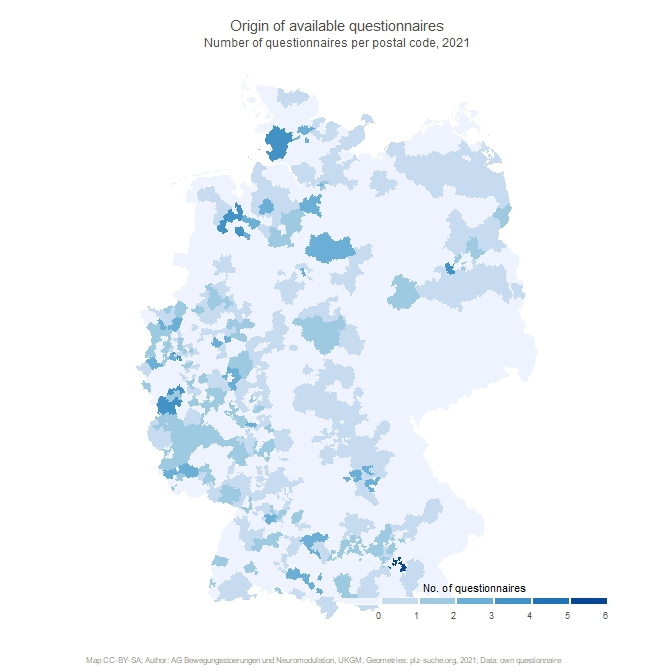
\includegraphics[width=.90\textwidth]{available.questionnaires.jpeg}
\label{fig1:questionnaires}
\end{subfigure}%
\begin{subfigure}[b]{0.35\linewidth}
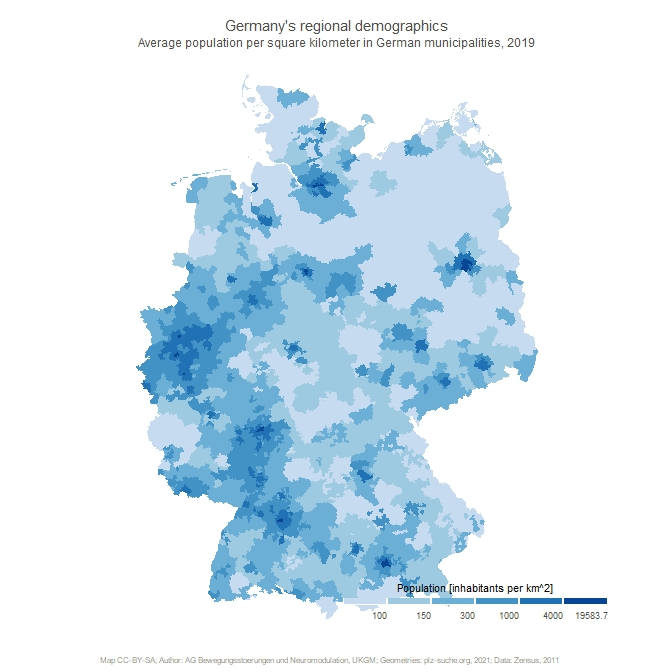
\includegraphics[width=.90\textwidth]{population.perskmGER.jpeg}
\label{fig1:population}
\end{subfigure}%
\begin{subfigure}[b]{0.35\linewidth}
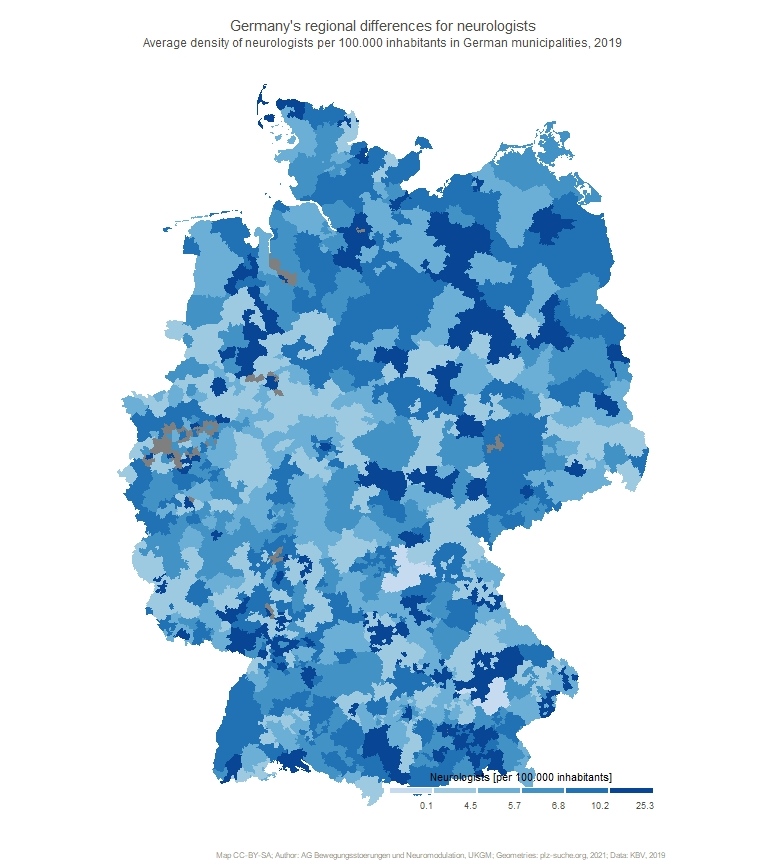
\includegraphics[width=.90\textwidth]{neurologists.10122021.jpeg}
\label{fig1:neurologists}
\end{subfigure}%
\caption{Demographic data for Germany and additional regional data for the obtained questionnaires. A) Number of received questionnaires within our survey for the distinct three digit postal codes. B) Illustration of inhabitants per square kilometer for Germany. C) Density of neurologists in all parts of Germany according to the German Statutory Health Insurance Association (\textit{Kassenärztliche Bundesvereinigung})}
\label{fig1:total}
\end{figure}

\begin{figure}[!h]
\centering
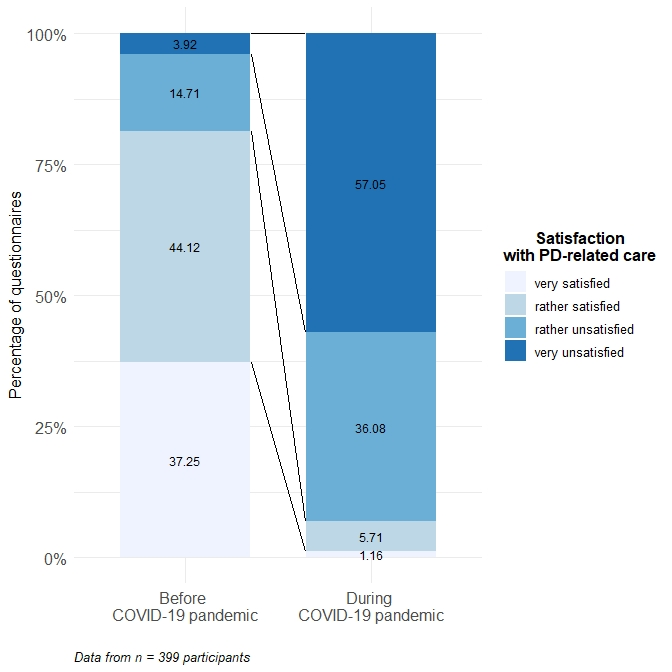
\includegraphics[width=.90\textwidth]{fig2.satisfaction.care.v1.0.jpeg}
\caption{B17 vs. C6 - Distribution of responses on the Satisfaction with PD-related care before and during the \textsc{Covid}-19 pandemic.}
\label{fig2:satisfaction}
\end{figure}

\begin{figure}[!h]
%Kann man die Grafik größer anzeigen und vielleicht sortieren?
%% DP: Wonach sortieren? Die Grafiken werden am Ende nicht eingefügt sondern als svg mitgeschickt, das Layout dürfen die übernehmen ;) 
\centering
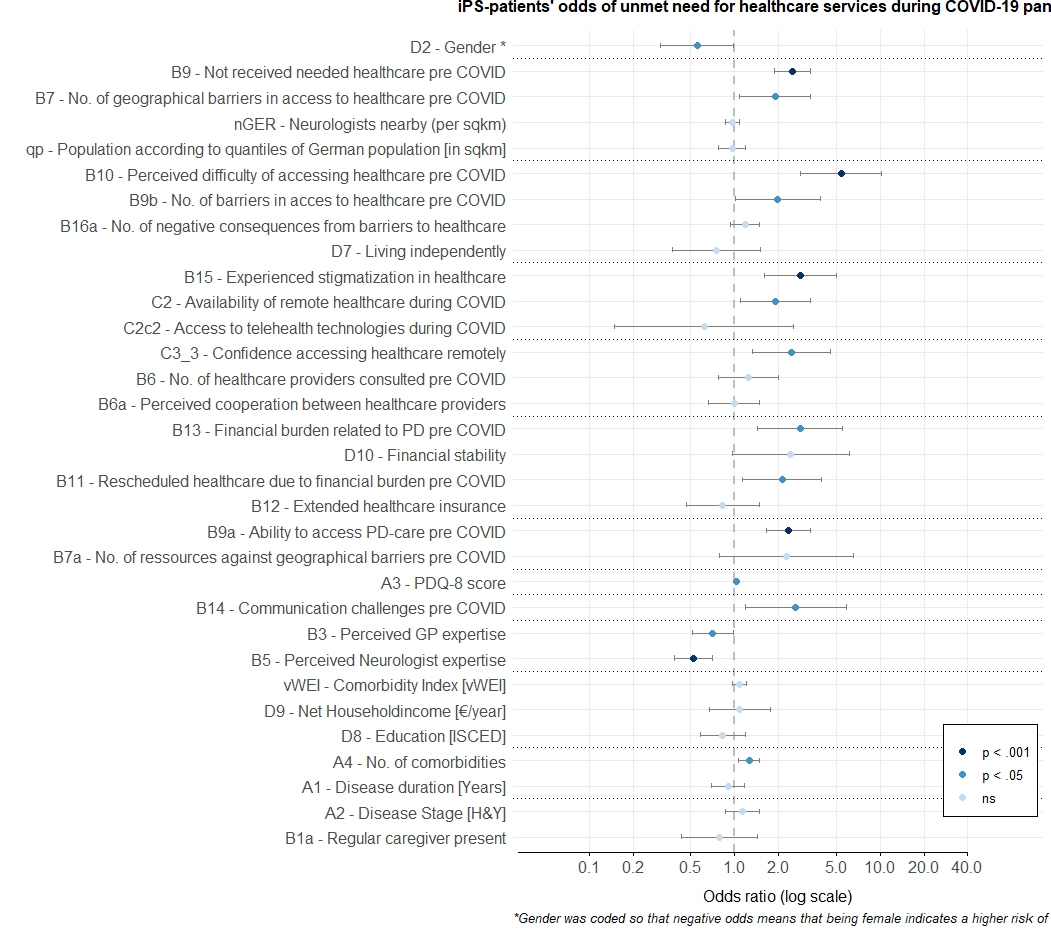
\includegraphics[width=\textwidth]{fig3.oddsratios.v1.0.jpeg}
\caption{Unadjusted Odds ratios according to the \ac{glm} for all 32 questions. Odds were determined so that higher values indicate affirmation to the question that healthcare was needed but this need remianed unmet during the \textsc{Covid}-19 pandemic. The dashed lines indicate the distinct domains according to Zaman et al. \cite{zaman2021barriers}, whereas significance is illustrated as color of the dot, with two distinct levels of significance. }
\label{fig3:resultsOR1}
\end{figure}

\begin{figure}[h!]
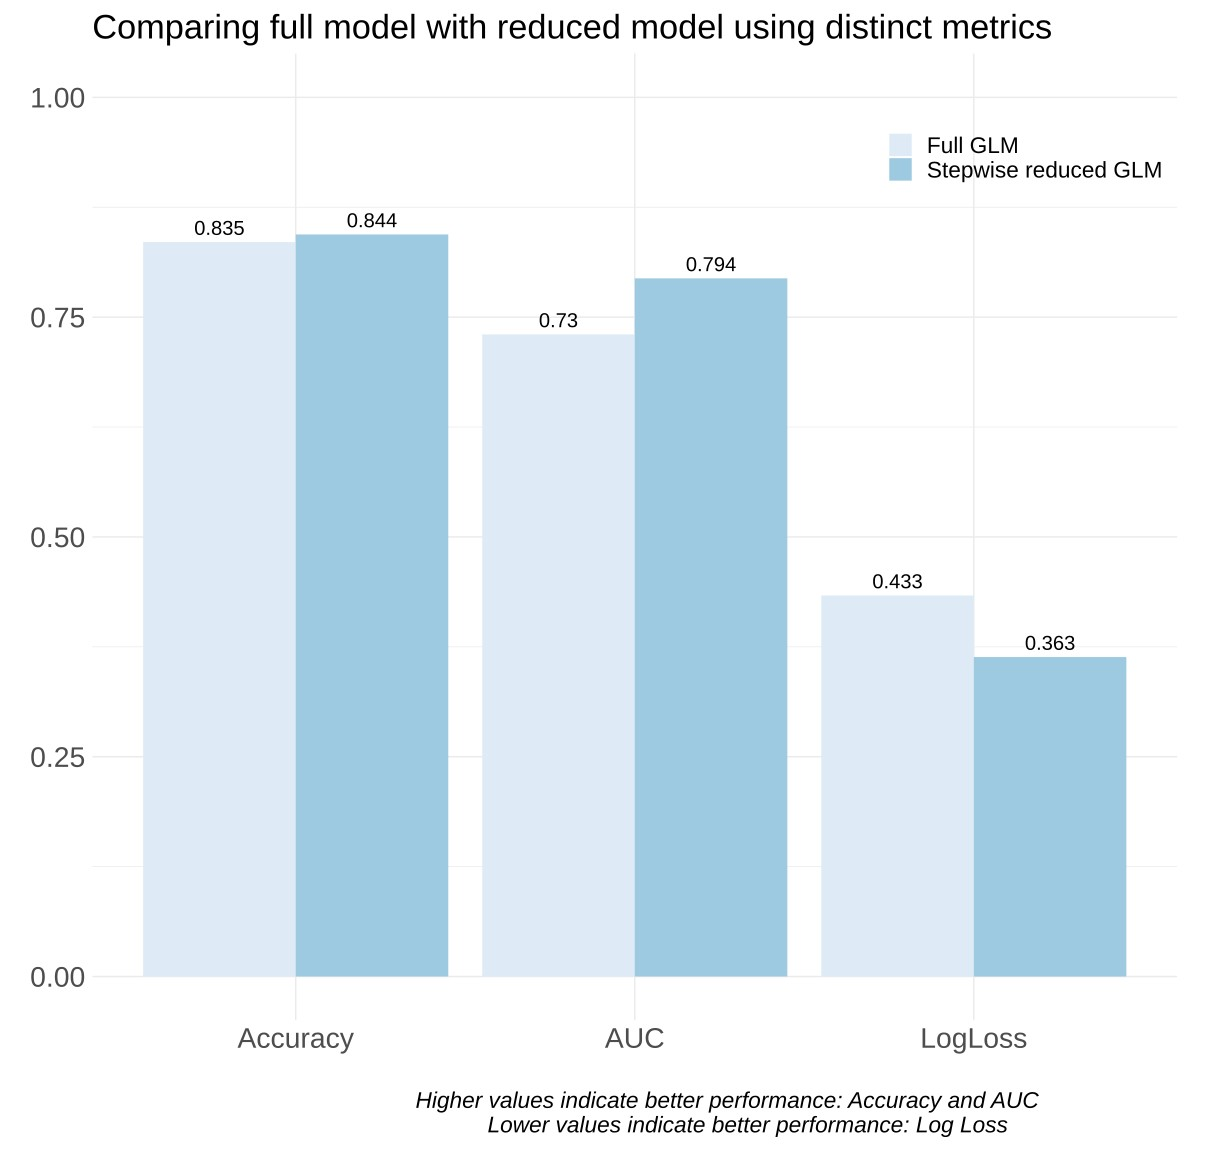
\includegraphics[width=.84\textwidth]{fig4.model.comparison.v1.0.jpg}
\caption{Comparison of the models. The full model including all 32 predictors was compatred in terms of accuracy to the reduced model resulting from the stepwise \ac{glm} regression. Values between both models are comparable although only 7 predictors remained in the model compared to the full model. For further details of the multilevel regression cf. Table \ref{tab2:reduced_model}}
\label{fig4:comparison_models}
\end{figure}

%%%%%%%%%%%%%%%%%%%%%%%%%%%%%%%%%%%
%%                               %%
%% Tables                        %%
%%                               %%
%%%%%%%%%%%%%%%%%%%%%%%%%%%%%%%%%%%

%% Use of \listoftables is discouraged.
%%
\newpage
\section*{Tables}
\begin{table}[!ht]
\caption{Demographics of subjects filling out questionnaire:}
\label{tab1:demographics}
\begin{tabular}{p{5cm} c}
\toprule
&\textbf{Overall}\\ %\hline
& \textbf{(n = 552)}\\ 
\midrule
Age (mean (SD)) & 66.76 (9.25) \\ \hline
Gender = female (\%) &  148 (41.6)  \\ \hline
Disease duration (\%) & \\ \hline
\hspace{3mm} $<$2 years & 62 (13.1) \\ \hline
\hspace{3mm} 2--5 years & 154 (32.6) \\ \hline
\hspace{3mm} 5--10 years & 157 (33.2) \\ \hline
\hspace{3mm} 10--15 years & 69 (14.6) \\ \hline
\hspace{3mm} $>$15 years& 31 ( 6.6) \\ \hline
Disease stage (\%)& \\ \hline
\hspace{3mm} Hoehn \& Yahr I &  189 (40.3) \\ \hline
\hspace{3mm} Hoehn \& Yahr II & 156 (33.3)  \\ \hline
\hspace{3mm} Hoehn \& Yahr III  &   77 (16.4) \\ \hline
\hspace{3mm} Hoehn \& Yahr IV  & 41 ( 8.7) \\ \hline
\hspace{3mm} Hoehn \& Yahr V  &     6 ( 1.3) \\ \hline
Education level according \newline to ISCED (\%) & \\ \hline
\hspace{3mm} primary education  & 20 ( 5.0) \\ \hline
\hspace{3mm} secondary education  & 234 (58.4)\\ \hline
\hspace{3mm} post secondary education  &   69 (17.2) \\ \hline
\hspace{3mm} highest education level possible & 78 (19.5)  \\ \hline
\hspace{3mm} PDQ-8 scores (mean (SD)) & 41.30 (14.23) \\ \hline
Van-Walraven-Elixhauser \newline \hspace{3mm} Comorbidity Index (mean (SD)) & 6.55 (1.95) \\ 
\bottomrule
\end{tabular}
\end{table}

\begin{table}[!ht]
\caption{Significant factors contibuting to unmet care needs during \textsc{Covid}-19 pandemic according to the reduced \ac{glm}:}
\label{tab2:reduced_model}
\centering
\begin{tabular}{l c c c c}
\toprule    
Predictor 												& Estimate 	& Std.Error & zvalue & \textit{p} \\
\midrule
(Intercept) 											& -2.65  		& 0.29 	& -9.24 	& $<$.0001 \\ \hline
Educational level (D8) 									& -0.73 		& 0.24 	& -3.01 	& 0.003 \\ \hline
Perceived GP's expertise (B3) 							& 0.34 		& 0.17 	& 2.07 	& 0.038 \\ \hline
Confidence in accessing necessary services remotely (C3) 	& 0.64 		& 0.22 	& 2.90 	& 0.004 \\ \hline
Ease obtaining healthcare prior to the pandemic (B10)		& -0.47 		& 0.22 	& -2.15 	& 0.031 \\ \hline
Ability to access care prior to the pandemic (B9)				& 0.41 		& 0.20 	& 2.07 	& 0.038 \\ \hline
Density of Neurologists 									& 0.47 		& 0.21 	& 2.22 	& 0.027 \\ \hline
Overcoming barriers (B7a)   								& -0.51 		& 0.22 	& -2.38 	& 0.017 \\
\bottomrule
\end{tabular}
\end{table}	


%%%%%%%%%%%%%%%%%%%%%%%%%%%%%%%%%%%
%%                               %%
%% Additional Files              %%
%%                               %%
%%%%%%%%%%%%%%%%%%%%%%%%%%%%%%%%%%%

\section*{Additional Files}
\begin{table}[!ht]
\caption{Matching of items in the questionnaire to the categories from the work of Zaman et al. \cite{zaman2021barriers}}
\label(tab3:matchingzaman)
\centering
\begin{tabular}{l l}
\toprule
\textbf{Question from \textsc{Covid}-Survey}& \textbf{Representative for what barrierer} \\
\midrule
1. A2, B1 & Autonomy \\ \hline
2. A1, A4, vWEI & Health Status \\ \hline
3. D8, D9 & Health Literacy \\ \hline
4. B3, B5 & Health Belief \\ \hline
5. B14a & Communication (personal) \\ \hline
6. PDQ-sum score & Self-efficacy \\ \hline
7. B7a, B9a/b & Transportation \\ \hline
8. B11, B12, B13, D10 & Cost of care \\ \hline
9. NA & Difficulties of Diagnosis \\ \hline
10. C3, B6a, B6 & Coordination in care \\ \hline
11. B15, B14, C2c & Communication (system) \\ \hline
12. B16, B16c, D6, D7, B9b, B10 & Disparty in Health Services \\ \hline
13. B7, B8, B9, & Unavailability of Specalist Services \\ \hline
14. D2 & Other \\
\bottomrule
\end{tabular}
\end{table}

\begin{table}[!ht]
\caption{Odds ratios for the distinct items of the questionnaire}
\label(tab4:resultsall)
\centering
\begin{tabular}{|p{5cm} | p{2cm} |l|l|l|l|}
\hline
\textbf{Factors} & \textbf{Domain} & \textbf{Odds Ratio} & \textbf{CIlower} & \textbf{CIupper} & \textbf{\textit{p}-value} \\ \hline
A2 - Disease Stage [H\&Y] & Autonomy & 1.13 & 0.87 & 1.47 & 0.367 \\ \hline
B1a - Regular caregiver present & Autonomy & 0.79 & 0.43 & 1.44 & 0.438 \\ \hline
A1 - Disease duration [Years] & Health Status & 0.9 & 0.69 & 1.16 & 0.419 \\ \hline
A4 - No. of comorbidities & Health Status & 1.26 & 1.06 & 1.49 & 0.007 \\ \hline
vWEI - Comorbidity Index [vWEI] & Health Belief & 1.08 & 0.97 & 1.21 & 0.155 \\ \hline
D8 - Education [ISCED] & Health Belief & 0.82 & 0.58 & 1.18 & 0.284 \\ \hline
D9 - Net Householdincome [per/year] & Health Belief & 1.08 & 0.67 & 1.75 & 0.75 \\ \hline
B3 - Perceived GP expertise & Health Literacy & 0.71 & 0.51 & 0.98 & 0.038 \\ \hline
B5 - Perceived Neurologist expertise & Health Literacy & 0.52 & 0.39 & 0.7 & p $<$ .001 \\ \hline
B14 - Communication challenges pre COVID & Communication (personal) & 2.63 & 1.18 & 5.82 & 0.017 \\ \hline
A3 - PDQ-8 score & Self-efficacy & 1.03 & 1.01 & 1.05 & 0.011 \\ \hline
B7a - No. of ressources against geographical barriers pre COVID & Transportation & 2.27 & 0.79 & 6.51 & 0.129 \\ \hline
B9a - Ability to access PD-care pre COVID & Transportation & 2.33 & 1.65 & 3.31 & p $<$ .001 \\ \hline
B11 - Rescheduled healthcare due to financial burden pre COVID & Cost of care & 2.11 & 1.13 & 3.93 & 0.019 \\ \hline
B12 - Extended healthcare insurance & Cost of care & 0.83 & 0.46 & 1.48 & 0.521 \\ \hline
B13 - Financial burden related to PD pre COVID & Cost of care & 2.81 & 1.42 & 5.53 & 0.003 \\ \hline
D10 - Financial stability & Cost of care & 2.43 & 0.97 & 6.09 & 0.059 \\ \hline
C3\_3 - Confidence accessing healthcare remotely & Difficulties of Diagnosis & 2.44 & 1.32 & 4.53 & 0.005 \\ \hline
B6a - Perceived cooperation between healthcare providers & Difficulties of Diagnosis & 0.99 & 0.66 & 1.49 & 0.975 \\ \hline
B6 - No. of healthcare providers consulted pre COVID & Difficulties of Diagnosis & 1.24 & 0.77 & 1.99 & 0.374 \\ \hline
B15 - Experienced stigmatization in healthcare & Coordination in care & 2.84 & 1.6 & 5.03 & p $<$ .001 \\ \hline
C2 - Availability of remote healthcare during COVID & Coordination in care & 1.91 & 1.09 & 3.34 & 0.023 \\ \hline
C2c2 - Access to telehealth technologies during COVID & Coordination in care & 0.62 & 0.15 & 2.53 & 0.5 \\ \hline
B16a - No. of negative consequences from barriers to healthcare & Communication (system) & 1.18 & 0.93 & 1.48 & 0.166 \\ \hline
D7 - Living independently & Communication (system) & 0.75 & 0.38 & 1.51 & 0.421 \\ \hline
B9b - No. of barriers in acces to healthcare pre COVID & Communication (system) & 1.98 & 1.01 & 3.89 & 0.048 \\ \hline
B10 - Perceived difficulty of accessing healthcare pre COVID & Communication (system) & 5.37 & 2.84 & 10.17 & p $<$ .001 \\ \hline
B7 - No. of geographical barriers in access to healthcare pre COVID & Disparty in Health Services & 1.9 & 1.08 & 3.33 & 0.026 \\ \hline
Population according to quantiles of German population [in sqkm] & Disparty in Health Services & 0.96 & 0.77 & 1.19 & 0.714 \\ \hline
B9 - Not received needed healthcare pre COVID & Disparty in Health Services & 2.5 & 1.88 & 3.32 & p $<$ .001 \\ \hline
nGER - Neurologists nearby (per sqkm) & Disparty in Health Services & 0.97 & 0.87 & 1.07 & 0.527 \\ \hline
D2 - Gender * & Unavailability of Specalist Services & 0.55 & 0.31 & 0.98 & 0.044 \\ \hline
\end{tabular}
\end{table}

\end{backmatter}
\end{document}
